\section{Convergencia de los tractogramas}

Recordemos el proceso de \textit{bootstraping} de la secci\'on \ref{sec:tractogramas}.
Creamos una poblaci\'on de \textit{streamlines} y luego estudiamos estad\'isticos
de sus subpoblaciones. Las Figuras \ref{fig:m1}, \ref{fig:m2} y \ref{fig:m3} 
muestran, para tres semillas distintas, cinco cortes coronales del tractograma 
creado usando quince mil \textit{streamlines}. Las Figuras \ref{fig:s1}, \ref{fig:s2}
y \ref{fig:s3} muestran la varianza de cada voxel dentro de un mismo corte
coronal para distintas cantidades de submuestras. \\

La Figura \ref{fig:mv} muestra la media y varianza de los voxels $A$, $B$ y $C$
marcados en las Figuras \ref{fig:s1}, \ref{fig:s2} y \ref{fig:s3}. Estos voxels
fueron los que mayor varianza presentaron al generar tractogramas usando 
subpoblaciones de dos mil \textit{streamlines}.\\


\begin{figure}[h!]
   \centering
    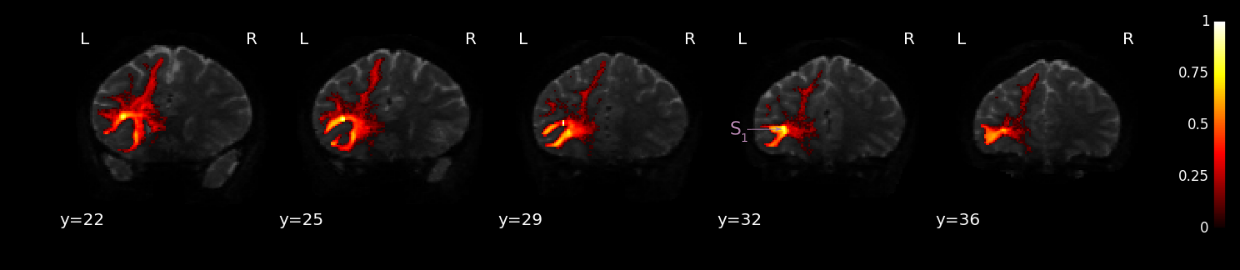
\includegraphics[width=0.9\textwidth]{img/m1.png}
    \caption{Tractograma para la semilla $S1$ utilizando toda la muestra.}
    \label{fig:m1}
\end{figure}

\begin{figure}[h!]
   \centering
    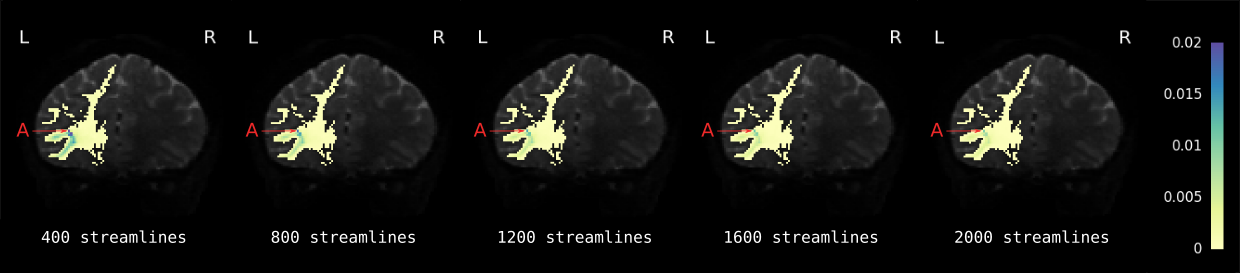
\includegraphics[width=0.9\textwidth]{img/s1.png}
    \caption{Desviaci\'on Estandar respecto a la semilla $S1$. Mismo corte axial
             variando el tama\~no de las submuestras.}
    \label{fig:s1}
\end{figure}

\begin{figure}[h!]
   \centering
    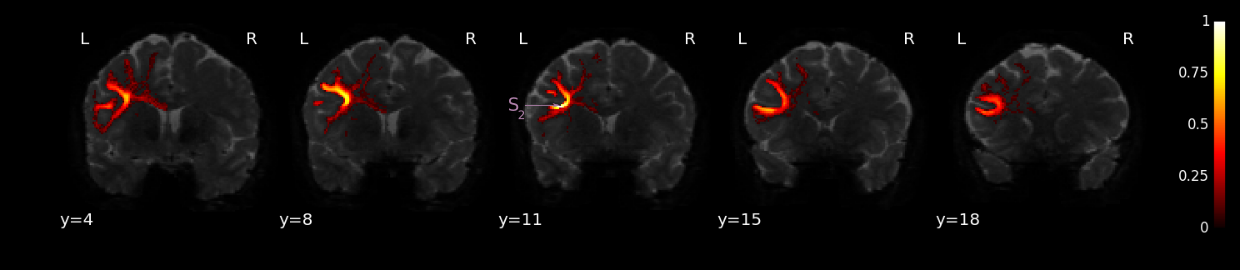
\includegraphics[width=0.9\textwidth]{img/m2.png}
    \caption{Tractograma para la semilla $S2$ utilizando toda la muestra.}
    \label{fig:m2}
\end{figure}

\begin{figure}[h!]
   \centering
    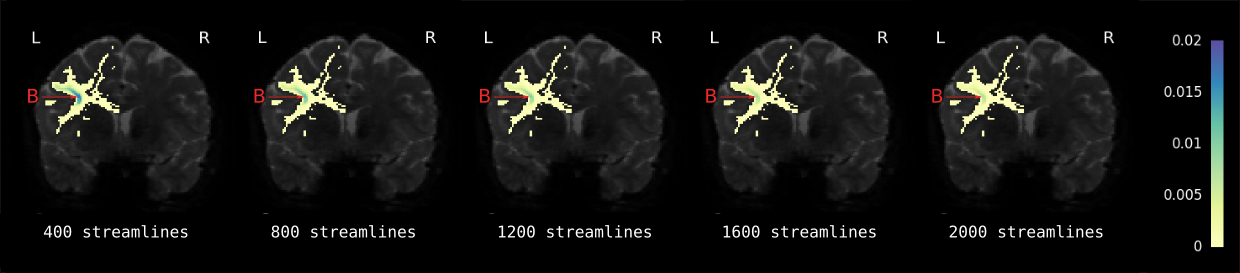
\includegraphics[width=0.9\textwidth]{img/s2.png}
    \caption{Desviaci\'on Estandar respecto a la semilla $S2$. Mismo corte axial
             variando el tama\~no de las submuestras.}
    \label{fig:s2}
\end{figure}

\begin{figure}[h!]
   \centering
    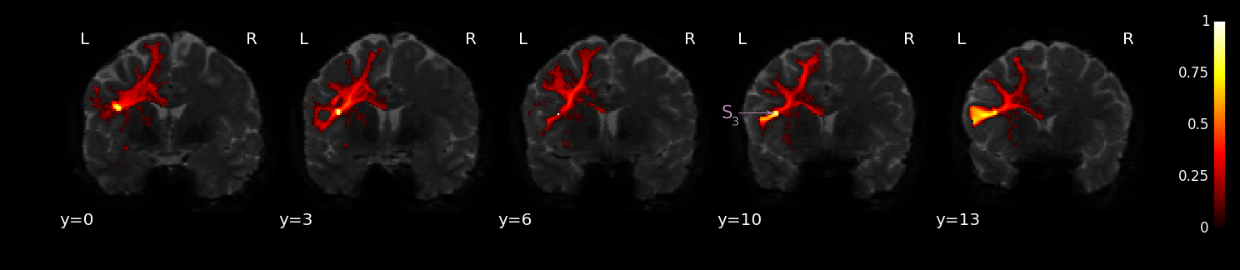
\includegraphics[width=0.9\textwidth]{img/m3.png}
    \caption{Tractograma para la semilla $S3$ utilizando toda la muestra}
    \label{fig:m3}
\end{figure}

\begin{figure}[h!]
   \centering
    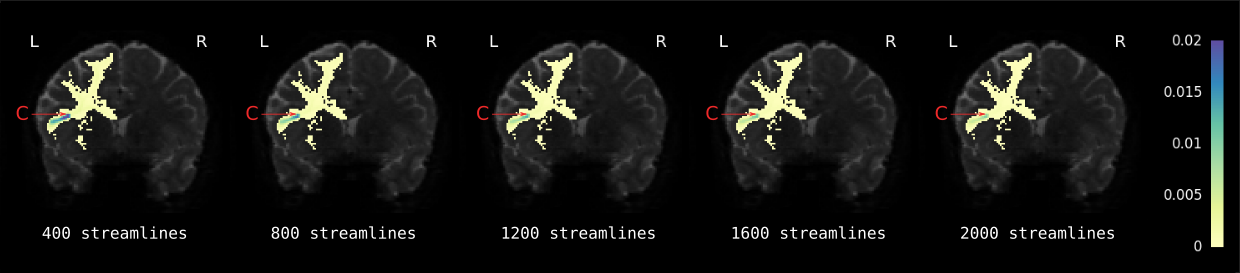
\includegraphics[width=0.9\textwidth]{img/s3.png}
    \caption{Desviaci\'on Estandar respecto a la semilla $S3$. Mismo corte axial
             variando el tama\~no de las submuestras.}
    \label{fig:s3}
\end{figure}

\begin{figure}[h!]
   \centering
    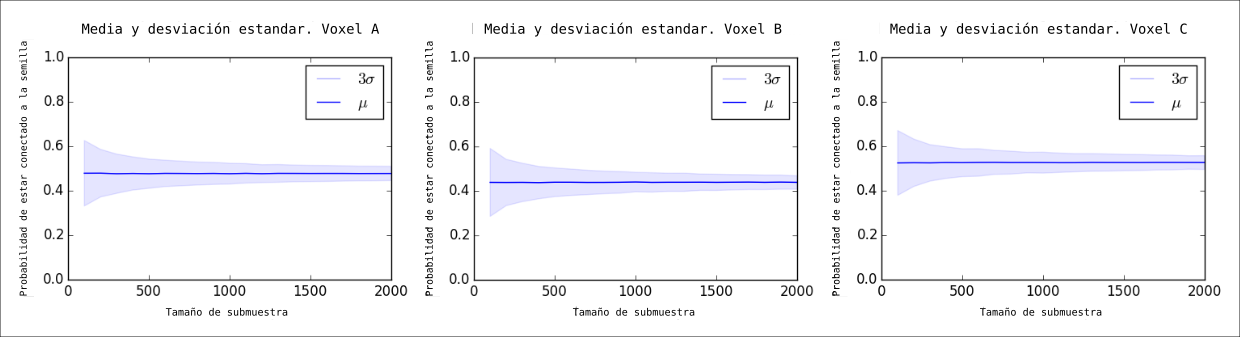
\includegraphics[width=0.9\textwidth]{img/med_var_all.png}
    \caption{Media y desviaci\'on estandar de los voxels con mayor varianza.}
    \label{fig:mv}
\end{figure}

\vspace{10cm}
